\documentclass[preprint,12pt,authoryear]{elsarticle}
\usepackage{amsmath,amssymb,booktabs,graphicx,xcolor,hyperref,multirow,siunitx}
\usepackage{adjustbox}
\hypersetup{colorlinks=true,linkcolor=blue!50!black,citecolor=blue!50!black,urlcolor=blue!50!black}
\sisetup{group-separator={,},group-minimum-digits=4}
% Placeholders for numbers that come from the GPU runs (Sec. 6). Search for \PH before submission.
\newcommand{\PH}[1]{\textcolor{red}{\textbf{[#1]}}}
\newcommand{\TODO}[1]{\textcolor{orange}{[TODO: #1]}}
\newcommand{\Sv}{S}
\newcommand{\Sl}{\tilde{S}}
\newcommand{\TVT}{\mathrm{TVT}}

\journal{Computers \& Geosciences}

\begin{document}
\begin{frontmatter}

\title{Learning the segment cost of a differentiable segment-Viterbi for true vertical thickness prediction in horizontal wells}

\author[kfupm]{Abdulrahman Al-Fakih\corref{cor1}}
\ead{abdulrahman.fakih@kfupm.edu.sa}
\author[amu]{Tabish Shah Mohsin}
\ead{email to be added}
\cortext[cor1]{Corresponding author.}
\affiliation[kfupm]{organization={College of Petroleum Engineering and Geosciences, King Fahd University of Petroleum and Minerals},
            city={Dhahran}, country={Saudi Arabia}}
\affiliation[amu]{organization={Department of Computer Engineering, Zakir Husain College of Engineering and Technology, Aligarh Muslim University},
            city={Aligarh}, country={India}}

\begin{abstract}
Geosteering keeps a horizontal well inside its target layer by locating the bit stratigraphically, expressed as the true vertical thickness (TVT) relative to a vertical reference well. We study automatic TVT prediction along the lateral from the trajectory, the lateral gamma-ray (GR) log and the typewell GR log, using the 773 labelled wells of the ROGII Kaggle competition. A data analysis first establishes the structure of the problem: over the evaluation zone the interpreted structural surface is piecewise linear (88\% of its length lies in straight pieces of 80\,ft or more), its slope relative to the trajectory trend stays within 0.05\,ft/ft over 98.6\% of the length, the GR misfit at the true position still leaves half of the GR variance unexplained, and 18\% of the wells admit a wrong constant shift that fits the GR within 30\% of the truth. We cast prediction as a shortest path on a lattice of straight segments in a coordinate detrended by the trajectory, score each candidate segment with a small convolutional network, add a learned transition cost that carries the interpreter's momentum relative to a neighbour-well structure field, and train both end-to-end through a soft-min (forward--backward) segment-Viterbi with a row-weighted squared-error loss. The lattice can represent the interpretations to within 0.42\,ft. In five-fold cross-validation the model reaches \PH{X.XX}\,ft RMSE against 15.91\,ft for holding the last known TVT, 14.55\,ft for following the trajectory trend and 11.80\,ft for the neighbour field alone, with \PH{N} trainable parameters; on the hidden test set it scores \PH{X.XXX}\,ft. Ablations isolate the contribution of the learned cost, the momentum term, the neighbour inputs and the corrected input scaling and loss weighting.
\end{abstract}

\begin{keyword}
Geosteering \sep True vertical thickness \sep Well-log correlation \sep Differentiable dynamic programming \sep Viterbi algorithm \sep Gamma ray
\end{keyword}

\begin{highlights}
\item Interpreted structure is piecewise linear; 98.6\% of it has slope $\le$0.05 vs.\ trend
\item TVT is predicted as a shortest path on a lattice of straight structural segments
\item Segment and transition costs are learned through a soft-min segment-Viterbi
\item Row-weighted loss and data-based input scaling fix two training biases
\item \PH{X.XX}\,ft cross-validated RMSE on 773 wells; code and weights released
\end{highlights}

\end{frontmatter}

%=====================================================================
\section{Introduction}\label{sec:intro}
A horizontal well is drilled to stay inside a thin target layer for thousands of feet. Because layers dip, fold and are offset by faults, the driller needs to know continuously where the bit is \emph{stratigraphically}, not only where it is in space. Geosteering answers this by correlating logs measured while drilling, most commonly the natural gamma ray (GR), with a vertical reference well (the \emph{typewell}). The interpreter adjusts the assumed geometry of the layers until the GR that the typewell predicts along the trajectory matches the GR that is measured. The result is the true vertical thickness (TVT) of every lateral sample: its vertical depth in the stratigraphic coordinate of the typewell.

Because the lateral log is recorded against measured depth (MD) while the typewell log is recorded against TVT, the task reduces to aligning two logs under geological constraints. The alignment is hard for three reasons that we quantify in Section~\ref{sec:data}. GR alone is a weak and periodic signal: even at the true position half of its variance is unexplained, and in a sizeable fraction of wells a wrong but consistent offset fits nearly as well as the truth. About a third of the lateral GR is missing. And errors compound: once an interpretation leaves the correct layer it rarely returns.

Commercial interpretation software builds the structure as a chain of joined straight segments, each placed by a geologist so that the implied GR matches the measured log \citep{rogii2026}. We take that construction literally. The prediction is a path on a lattice of straight segments in a coordinate detrended by the trajectory (Section~\ref{sec:lattice}), and the best path is found by dynamic programming \citep{viterbi1967,forney1973}, the classical tool for well-log alignment \citep{sakoe1978,wheeler2015}. What a hand-written alignment cost cannot express is \emph{which} of several GR-consistent paths a geologist would choose. We therefore learn the cost: a small network scores each candidate segment from the GR, the typewell, the segment geometry and a neighbour-well structure field, and a transition network adds the interpreter's tendency to persist in his deviation from the neighbours. Both are trained \emph{through} the dynamic program by replacing the minimum with a soft minimum \citep{mensch2018diffdp,cuturi2017softdtw}, so that the expected path, not a surrogate label, is fitted to the interpreted TVT.

\paragraph{Contributions}
\begin{enumerate}
\item A quantitative analysis of the ROGII training interpretations (Section~\ref{sec:data}): segment lengths and slopes of the interpreted surface, with and without detrending by the trajectory; fault frequency and size; the information content and ambiguity of GR at the true position; the spatial layout of the wells; and baselines from trivial to oracle. Each design constant of the method is tied to one of these measurements.
\item A second-order soft segment-Viterbi whose segment and transition costs are small neural networks trained end-to-end on the TVT error (Section~\ref{sec:method}). The lattice resolution costs 0.42\,ft RMSE; the cost network has \PH{N} parameters.
\item Two corrections of the training procedure that matter for this data: inputs standardized with statistics measured on the data (the earlier scaling left the neighbour input ten times wider than the GR inputs and a misfit clip that never acted), and a loss that weights every predicted row equally across batches (Section~\ref{sec:train}).
\item Five-fold cross-validated results with ablations, hidden-test scores and an error analysis (Section~\ref{sec:results}); code, configurations, notebooks and weights are released (Section~\ref{sec:code}).
\end{enumerate}

%=====================================================================
\section{Related work}\label{sec:related}
\paragraph{Well-log correlation and geosteering}
Aligning logs by dynamic programming goes back to dynamic time warping \citep{sakoe1978}; for well logs it has been extended to the simultaneous correlation of many wells \citep{wheeler2015}. In geosteering the stratigraphic position is usually tracked sequentially. \citet{veettil2020} estimate it with sequential Monte Carlo, \citet{alyaev2019} combine an ensemble of geological realizations with decision support, and \citet{muhammad2025} couple a particle filter with a reinforcement-learning agent that also chooses the steering. These methods operate while drilling and model the uncertainty explicitly; our task is the offline completion of an interpretation, scored by squared error.

\paragraph{The ROGII competition}
The data and task come from a Kaggle competition \citep{rogii2026}. The strongest published solutions are dense image models: the winning solution aligns the lateral against the typewell with a two-dimensional (lateral position $\times$ candidate depth) U-Net \citep{ronneberger2015unet} on a pretrained ConvNeXt encoder \citep{liu2022convnext}, with particle-filter and neighbour-well channels, synthetic training wells and a large ensemble \citep{rogii1st}. The second-place solution predicts a distribution of moves on an anchor grid with a convolutional network and decodes it by dynamic programming; the third combines hidden Markov models with a particle filter and a gating network \citep{rogiiforum}. The piecewise-linear character of the interpreted structure was also noted in the competition forum \citep{rogiiforum}. In all of these the structural decoding, when present, is a fixed post-process of a network trained with a classification or regression loss. Here the decoder is part of training.

\paragraph{Differentiable dynamic programming}
Replacing $\min$ by a smoothed minimum makes a dynamic program differentiable \citep{mensch2018diffdp}; soft-DTW is the best known instance \citep{cuturi2017softdtw}. Conditional random fields \citep{lafferty2001crf} train the potentials of a chain model through its partition function, and hidden Markov models compute posterior marginals with the same forward--backward recursion \citep{rabiner1989}. We use the soft-min forward--backward recursion to obtain the \emph{posterior-mean} path and fit it to the target with a squared-error loss, which matches the evaluation metric.

%=====================================================================
\section{Data and problem analysis}\label{sec:data}
\subsection{Task and data}
Each well provides a lateral table sampled every foot of MD with the trajectory ($X$, $Y$ and the vertical coordinate $Z$, which is negative below sea level), the lateral GR and \texttt{TVT\_input}, which holds the interpreted TVT up to row $K$ (the \emph{known section}) and is missing afterwards. A typewell table gives GR against TVT. The target is the TVT of rows $K,\dots,N-1$ (the \emph{prediction zone}), scored by the root-mean-square error (RMSE) pooled over all predicted rows of all wells. The trajectory is known over the whole well, including the prediction zone. The 773 training wells carry the full interpreted TVT; the scored test wells are hidden (the three public test wells are copies of training wells).

A typical well has \num{6576} rows (10th--90th percentile \num{4993}--\num{8056}), of which \num{1703} are known and \num{4840} (\num{3263}--\num{6349}) must be predicted, about 74\% of the well (Fig.~\ref{fig:well}). The training set has \num{3783989} predicted rows. Because the metric pools rows, long wells weigh more: the longest 20\% of the wells hold 27\% of the scored rows. The lateral GR is missing on 31.5\% of the prediction-zone rows (median well 30\%, 90th percentile 60\%) and on 23.6\% of the known rows; the typewell GR is complete. Wells whose typewells share more than half of their samples form 54 typewell families (13 with a single well, the largest with 71 wells).

\begin{figure}[!htbp]\centering
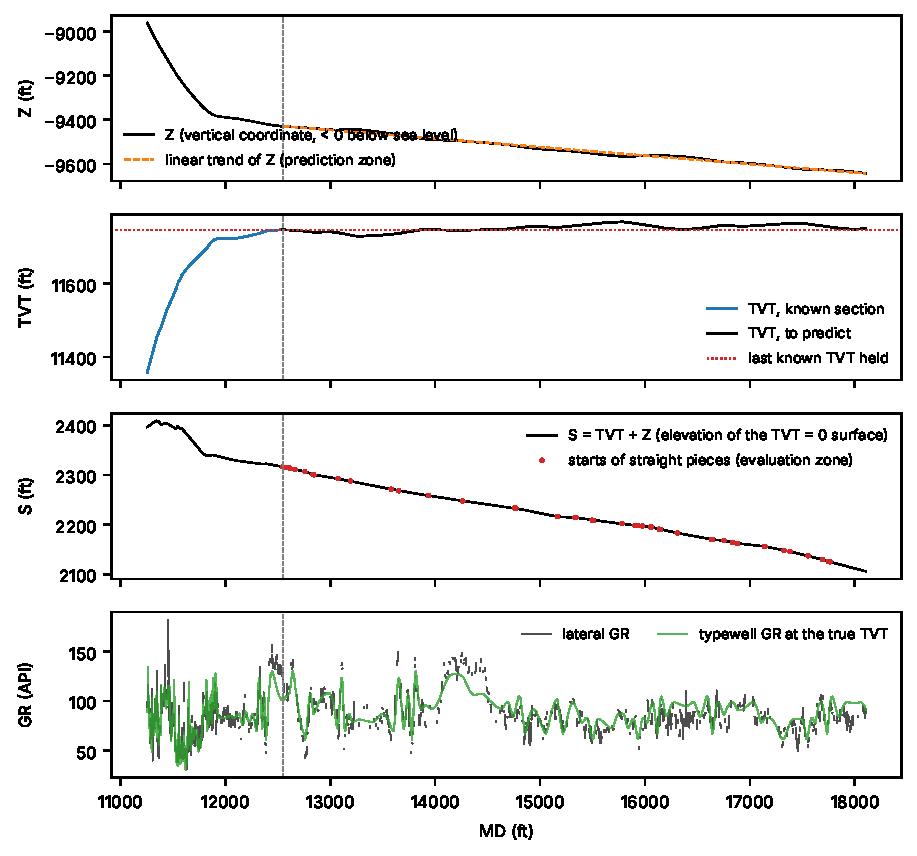
\includegraphics[width=\linewidth]{figures/well_example.pdf}
\caption{One training well (01869cd4). From top: true vertical depth $Z$ and its linear trend over the prediction zone; TVT, known (blue) and to be predicted (black), with the last known value held; $\Sv=\TVT+Z$, the elevation of the TVT\,=\,0 surface (Section~\ref{sec:tvt}), with the starts of the straight pieces of the evaluation zone; the lateral GR and the typewell GR read at the true TVT. The dashed line marks the end of the known section.}\label{fig:well}
\end{figure}

\subsection{What TVT measures}\label{sec:tvt}
The task description defines TVT as depth in the vertical typewell \citep{rogii2026}. The data show precisely what this means for a lateral sample: its TVT is the depth below the typewell's zero at which the same rock is found. Three checks on all training wells support this. The TVT at which a lateral lies exactly on a formation top equals the TVT at which the typewell's formation label of that top begins (\num{2383} well--top pairs, median difference $-0.2$\,ft, one typewell sample). Wells that share a typewell assign the identical TVT to each top. And $\TVT+Z$ minus the elevation of any top, both given along the lateral, is constant along each well to within 0.007\,ft.

The level TVT\,=\,0 can therefore be carried from the typewell into the section parallel to the layers (Fig.~\ref{fig:tvt}). TVT is the depth of the bit below this surface, $Z$ is the elevation of the bit and
\begin{equation}
\Sv = \TVT + Z
\end{equation}
is the elevation of the TVT\,=\,0 surface relative to sea level at the bit, with no further constant. Its sign carries no meaning: it depends only on where the typewell's zero lies. Its per-well median lies between \num{1499} and \num{2542}\,ft (median 2110\,ft). The typewell files contain only the logged interval, which starts \num{9976}--\num{11908}\,ft below the zero (5th--95th percentile), so TVT values are never near zero. Neither the datum of the typewell nor its location is given; the analysis needs neither.

\begin{figure}[!htbp]\centering
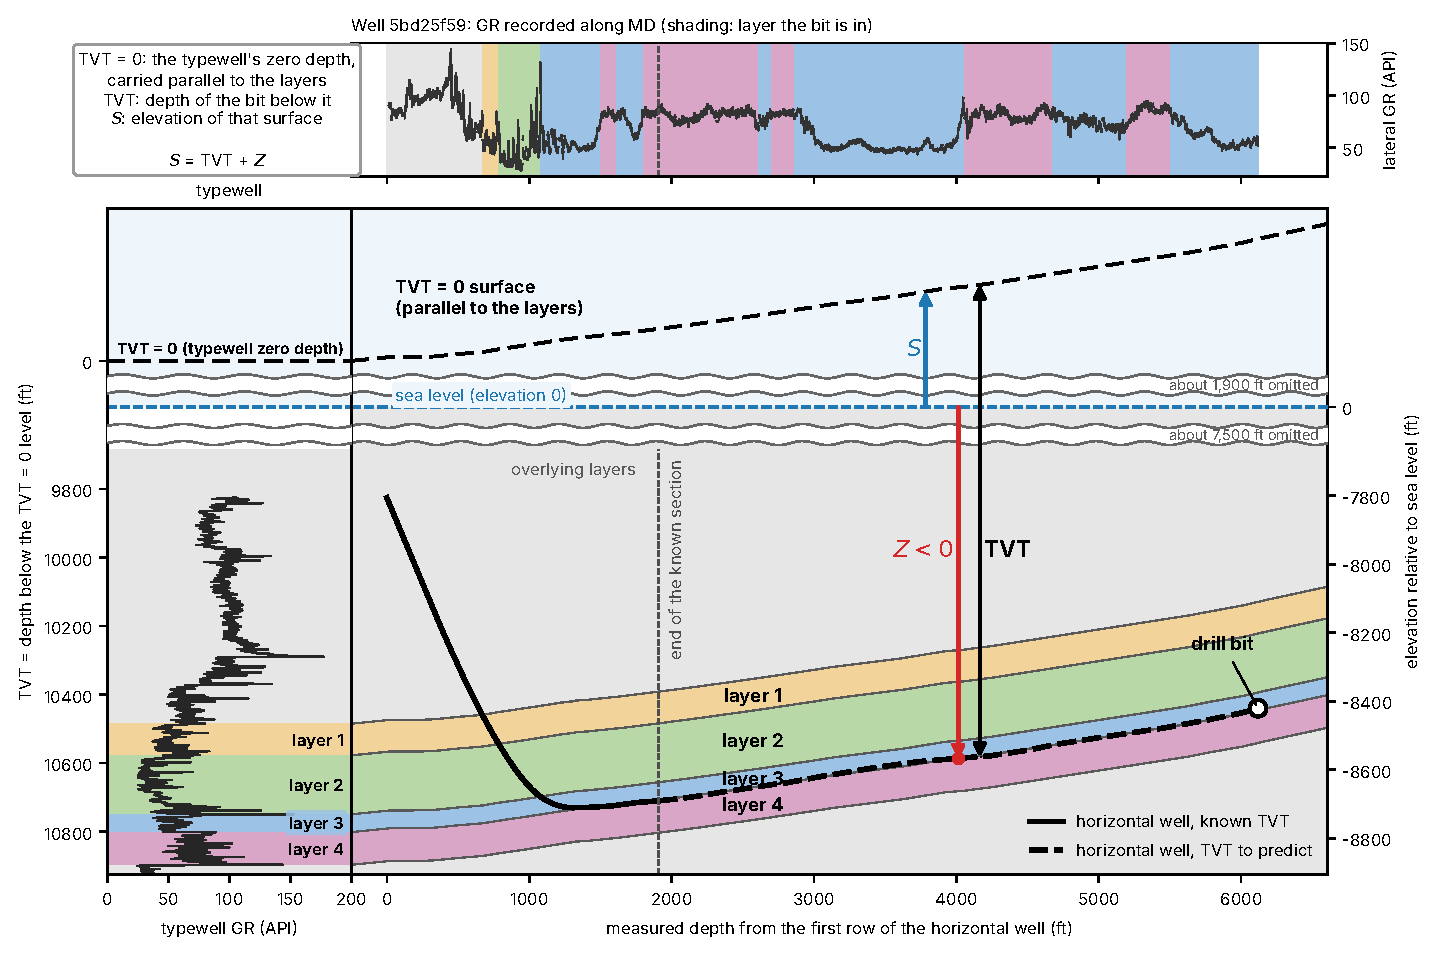
\includegraphics[width=\linewidth]{figures/s_tvt_z.pdf}
\caption{What TVT measures, drawn from the data of training well 5bd25f59 (four of its formation tops shown as layers 1--4; vertical exaggeration about 3$\times$; two axis breaks omit about 7{,}500\,ft between the layers and sea level and about 1{,}900\,ft between sea level and the TVT\,=\,0 surface). Left: the typewell, GR against TVT; TVT\,=\,0 is its zero depth. Main panel: the horizontal well in elevation, with the TVT\,=\,0 level carried parallel to the layers (dashed). At a point in the middle of the section to predict, TVT is the depth of the well below that surface, $Z$ its elevation and $\Sv=\TVT+Z$ the elevation of the surface (positive for this well because the surface lies above sea level). Top: the lateral GR, shaded by the layer the bit is in.}\label{fig:tvt}
\end{figure}

\subsection{The interpreted structure is piecewise linear}\label{sec:pwl}
Because the TVT\,=\,0 surface is parallel to the layers, $\Sv$ along the trajectory traces the interpreted structure: it is constant where the layers are flat and changes with their dip. We analyse it over the evaluation zone only (the rows without \texttt{TVT\_input}), where the labels are the interpreter's piecewise construction; in the known section they follow the build of the well. TVT and $Z$ are stored to 0.01\,ft, so $\Sv$ carries a rounding error of up to $\pm0.01$\,ft and differences of consecutive rows stagger by up to 0.02\,ft (a true increment of $-0.038$\,ft per row appears as $-0.03$, $-0.04$ and $-0.05$). We therefore never take slopes or jumps from consecutive rows. Instead, the evaluation zone of every well is cut into the fewest consecutive pieces such that a least-squares line fits every row of a piece within 0.015\,ft, just above the rounding bound (a greedy longest-piece search, which is optimal for this criterion). The residuals inside the pieces are then pure rounding noise, while a tolerance of 0.03\,ft already merges real changes of dip. Measuring along MD, along the cumulative horizontal distance or along the vertical section gives the same pieces. At each junction we evaluate the two neighbouring lines midway between the last row of one piece and the first row of the next: their difference is the offset at the junction and the difference of their slopes the change of dip, so that each junction is counted once.

The 773 evaluation zones (\num{3783989} rows) give \num{29394} pieces, 35 per well (median), with a broad length distribution (median 76\,ft, 10th--90th percentile 11--319\,ft; Table~\ref{tab:segments}, Fig.~\ref{fig:segments}). Pieces of 80\,ft or more cover 87.8\% of the length and pieces of 200\,ft or more 59.9\%. Short pieces are steeper: the 90th percentile of the detrended slope is 0.039 for pieces of 10--40\,ft and 0.022 for pieces of 200--500\,ft, which matches the short, sharper corrections an interpreter makes between long runs.

\begin{table}[!htbp]\centering\small
\caption{Straight pieces of the interpreted surface over the evaluation zones of the 773 training wells (least-squares pieces, tolerance 0.015\,ft). Slopes are $|d\Sv/d\mathrm{MD}|$, raw and relative to the linear trend of $Z$ over the evaluation zone.}\label{tab:segments}
\begin{adjustbox}{max width=\linewidth}
\begin{tabular}{lrrcc}
\toprule
Piece length (ft) & Pieces & Share of length & \multicolumn{2}{c}{$|$slope$|$ median / 90th / 99th pct.} \\
\cmidrule(lr){4-5}
 & & & raw & detrended \\
\midrule
$<10$     & \num{1922} & 0.4\%  & 0.035 / 0.065 / 0.114 & 0.011 / 0.041 / 0.111 \\
10--40    & \num{8378} & 4.5\%  & 0.034 / 0.063 / 0.112 & 0.012 / 0.039 / 0.096 \\
40--80    & \num{4774} & 7.4\%  & 0.034 / 0.064 / 0.102 & 0.013 / 0.038 / 0.078 \\
80--200   & \num{8123} & 27.9\% & 0.033 / 0.059 / 0.093 & 0.011 / 0.030 / 0.059 \\
200--500  & \num{5170} & 41.2\% & 0.033 / 0.053 / 0.076 & 0.008 / 0.022 / 0.044 \\
$\ge 500$ & \num{1025} & 18.7\% & 0.033 / 0.048 / 0.066 & 0.006 / 0.017 / 0.033 \\
\bottomrule
\end{tabular}
\end{adjustbox}
\end{table}

\begin{figure}[!htbp]\centering
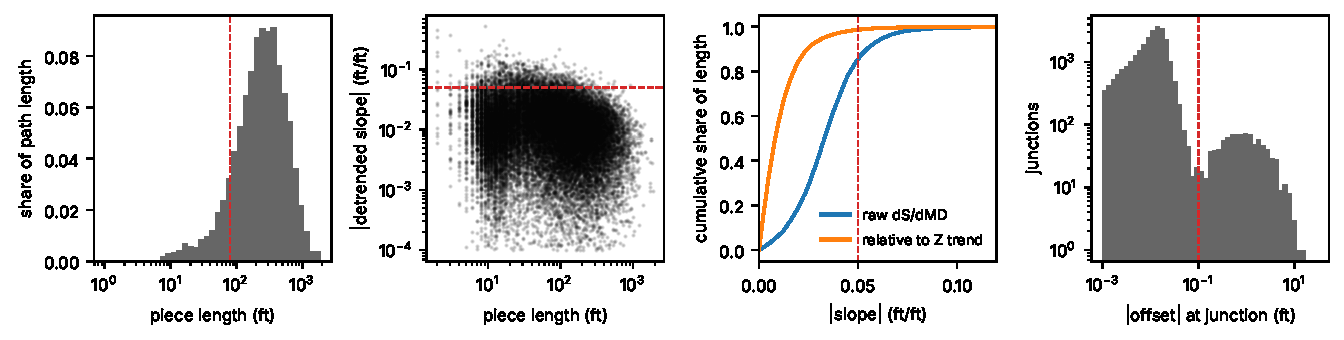
\includegraphics[width=\linewidth]{figures/segments.pdf}
\caption{Straight pieces of the interpreted surface (prediction zones, all training wells). Left: distribution of piece length, weighted by length; the dashed line is the 80-ft chunk of the lattice. Second: detrended slope against length. Third: share of the path length whose slope is below a given value, raw and relative to the $Z$ trend; the dashed line is the slope limit of the lattice. Right: offsets between neighbouring pieces at their junctions; the gap near 0.1\,ft separates continuous junctions (rounding, $\lesssim$0.05\,ft) from faults.}\label{fig:segments}
\end{figure}

\paragraph{Detrending by the trajectory}
The raw slope of $\Sv$ is dominated by the well's own inclination: the slope of the linear trend of $Z$ ranges from $-0.045$ to $0.049$ (5th--95th percentile) between wells. Measured relative to that trend, 98.6\% of the path length has a slope of at most 0.05\,ft/ft and 93.8\% at most 0.03, against 85.3\% and 41.7\% for the raw slope (Fig.~\ref{fig:segments}, right). In other words the layers run nearly parallel to the trajectory's mean direction, which is how the well was planned. The same effect appears in the baselines (Table~\ref{tab:baselines}): holding $\TVT+Z$ constant (flat layers) gives 107.5\,ft RMSE, holding TVT constant gives 15.91\,ft, and holding $\Sv$ constant relative to the $Z$ trend gives 14.55\,ft. The trend captures the slow drift; the residual departures of $Z$ from its line (the steering corrections) are what the detrended coordinate removes from $\Sv$. We therefore build the lattice in the detrended coordinate with a slope limit of 0.05.

\paragraph{Faults}
In this construction a fault is an offset between two consecutive pieces. The offsets at the \num{28621} junctions are clearly bimodal (Fig.~\ref{fig:segments}, right): \num{27597} are below 0.05\,ft, i.e.\ continuous within rounding, only 114 lie between 0.05 and 0.1\,ft, and 910 exceed 0.1\,ft. We call the latter faults. They occur in 40.6\% of the wells, about one per 4\,kft of evaluation zone; their size has median 0.79\,ft, 90th percentile 3.1\,ft and 99th percentile 8.1\,ft. A fault larger than 1, 2, 5 and 10\,ft occurs in 26.8\%, 15.8\%, 3.6\% and 0.3\% of the wells. Faults are therefore common but mostly small relative to the error levels in this study. The lattice does not model them explicitly; a fault of a few feet becomes a steeper segment over one chunk, and the cost of that approximation is included in the lattice oracle below.

\subsection{How informative and how ambiguous is GR?}\label{sec:gr}
We standardize GR with the global mean and standard deviation of the low-pass lateral GR of the training wells (88.2 and 23.4\,API). Along the \emph{true} path, the lateral GR differs from the reference GR by 10.0\,API RMS (median absolute 5.6, 90th percentile 15.9, 99th percentile 31.0\,API) when the reference blends the typewell with the well's own known section (Section~\ref{sec:inputs}), and by 11.0\,API with the typewell alone. Even at the truth, 51\% of the lateral GR variance in the prediction zone is unexplained (61\% with the typewell alone).

To measure ambiguity we shifted the whole true path by a constant $\delta$ with $5\le|\delta|\le30$\,ft and compared the best shifted misfit with the misfit of the truth. For 18.1\% of the wells some wrong shift fits within 30\% of the truth's misfit, and for 8.7\% a wrong shift fits \emph{better} than the truth (27.4\% and 14.0\% with the typewell alone). GR alone cannot resolve these wells; the decision must come from geology (continuity, typical dips, neighbouring wells), which is what the learned costs provide.

\subsection{Spatial layout and validation protocol}\label{sec:spatial}
The wells cover an area of about 34 by 24 miles, mostly in pads of parallel laterals (Fig.~\ref{fig:map}). The median distance from a lateral to the nearest other well is 364\,ft (10th--90th percentile 172--1004\,ft). We validate with a random five-fold split by well (sorted names, permutation seed 42, fold = position modulo 5). Under this split the nearest well of another fold is almost as close (median 398\,ft) as the nearest well overall, so the cross-validation measures interpolation between neighbouring wells. The hidden test wells come from the same field; the gains that the top solutions report from neighbour-well inputs suggest that they are also interleaved with the training wells, but this cannot be verified from the public data. All neighbour inputs of a training well are computed from the other folds only.

\begin{figure}[!htbp]\centering
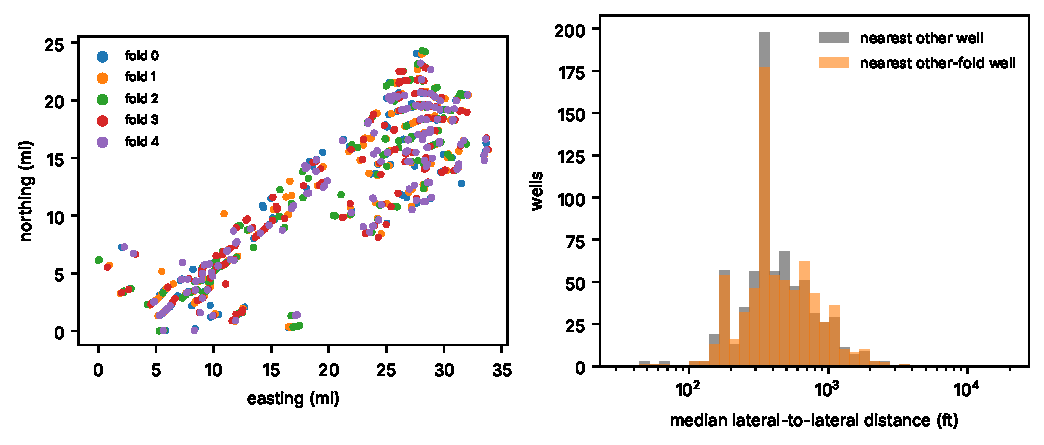
\includegraphics[width=\linewidth]{figures/map.pdf}
\caption{Left: well locations (median of each lateral) coloured by cross-validation fold. Right: median distance from each lateral to the nearest other well and to the nearest well of another fold.}\label{fig:map}
\end{figure}

\subsection{Baselines and the lattice oracle}\label{sec:baselines}
Table~\ref{tab:baselines} lists reference predictors evaluated on all 773 training wells. The neighbour field (Section~\ref{sec:inputs}) predicts the TVT from the structure of the other-fold wells alone (11.80\,ft); projecting the single nearest well's surface, anchored at the last known row, is much worse (23.83\,ft), because levels do not transfer between wells while shapes do: for pairs of wells of the same typewell family that run within 400\,ft of each other over at least 1.5\,kft, 81.5\% of the squared difference between their surfaces is a constant offset (median 7.9\,ft), 9.7\% a linear drift (median 2.0\,ft/kft) and 8.8\% a residual (median 3.0\,ft RMS). The \emph{lattice oracle} is the best path of our lattice given the truth (an exact dynamic program on the squared error); its 0.42\,ft shows that the lattice itself is not a limitation (only 11 wells exceed 1\,ft and one exceeds 3\,ft, at 5.6\,ft). Holding the last TVT scores 14.488\,ft private / 15.883\,ft public on the hidden test set, close to its cross-validated 15.91\,ft.

\begin{table}[!htbp]\centering\small
\caption{Baselines on the prediction zones of the 773 training wells (pooled RMSE, ft) and per fold. Leaderboard: hidden test, private / public.}\label{tab:baselines}
\begin{adjustbox}{max width=\linewidth}
\begin{tabular}{lrcl}
\toprule
Predictor & RMSE & per fold (0--4) & Leaderboard \\
\midrule
Hold last known TVT & 15.91 & 17.7 / 15.7 / 14.6 / 14.7 / 16.6 & 14.488 / 15.883 \\
Flat layers ($\TVT+Z$ constant) & 107.5 & 109 / 108 / 111 / 104 / 105 & \\
Extrapolate TVT trend of last 300\,ft & 130.2 & & \\
Layers parallel to the $Z$ trend & 14.55 & 15.1 / 14.6 / 13.2 / 13.7 / 16.1 & \PH{} \\
Nearest-well surface, anchored & 23.83 & 25.0 / 31.9 / 23.5 / 16.2 / 19.4 & \\
Neighbour structure field & 11.80 & 12.2 / 11.1 / 10.9 / 12.4 / 12.3 & \PH{} \\
Viterbi with hand-crafted GR cost & \PH{} & \PH{} & \\
\midrule
Lattice oracle (truth known) & 0.42 & 0.33 / 0.63 / 0.28 / 0.31 / 0.46 & \\
\bottomrule
\end{tabular}
\end{adjustbox}
\end{table}

%=====================================================================
\section{Method}\label{sec:method}
\subsection{Detrended coordinate and segment lattice}\label{sec:lattice}
Let $Z_{\mathrm{lin}}$ be the least-squares line of $Z$ against MD over the lattice rows and $z_{\det}=Z_{\mathrm{lin}}-Z$. The lattice coordinate of a TVT value is
\begin{equation}
\Sl = \TVT - \mathrm{off},\qquad \mathrm{off}(i) = \TVT(s) + z_{\det}(i) - z_{\det}(s),
\end{equation}
so that $\Sl=0$ at the first lattice row $s$. Up to a constant, $\Sl=\Sv-Z_{\mathrm{lin}}$: the TVT\,=\,0 surface measured relative to the trajectory trend, and $\Sl\equiv$ const describes layers parallel to that trend. The lattice starts $r$ rows before the end of the known section, with $r$ chosen so that chunks of $D=80$ rows end exactly at the last row of the well ($1\le r\le D$); the first chunk therefore overlaps the known section, and the path starts from the known TVT. At every chunk boundary the anchors are the integers $a\in[-K_C,K_C]$ with $K_C=100$\,ft. A candidate segment joins anchor $a$ at one boundary to $a+m$ at the next with $|m|\le M_V=\mathrm{round}(0.05\,D)=4$, the slope limit of Section~\ref{sec:pwl} (Fig.~\ref{fig:lattice}). Each chunk thus has $201\times 9$ candidate segments. The prediction is the straight-line interpolation of the chosen anchors, mapped back by $\TVT=\Sl+\mathrm{off}$. The choice $D=80$ trades lattice resolution against the length of GR evidence per segment; with 88\% of the interpreted path in pieces of at least 80\,ft, the oracle error is 0.42\,ft.

\begin{figure}[!htbp]\centering
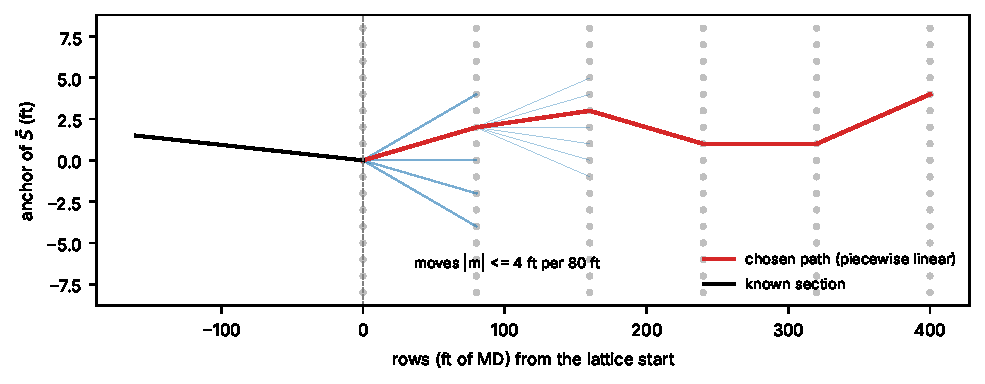
\includegraphics[width=0.85\linewidth]{figures/lattice.pdf}
\caption{The segment lattice (schematic, reduced anchor range). Anchors (grey) sit at chunk boundaries 80 rows apart; each anchor connects to the 9 anchors within $\pm4$\,ft at the next boundary (blue, shown for two anchors); a path (red) is a chain of straight segments starting from the known section.}\label{fig:lattice}
\end{figure}

\subsection{Inputs of a candidate segment}\label{sec:inputs}
For a candidate segment we extend its line by two chunks backwards and two forwards and sample it at $16$ points per chunk ($N_P=80$ points). At each point the network sees seven channels:
\begin{itemize}
\item $g$, the lateral GR (missing values interpolated, first-order Butterworth low-pass, 5-row box average), standardized with the global GR statistics;
\item $t$, the reference GR at the TVT implied by the line, standardized the same way; the reference is the typewell GR blended (weight 0.7) with the well's own known-section GR binned by its known TVT within $\pm100$\,ft of the last known TVT (the blend reduces the misfit at the truth from 11.0 to 10.0\,API and the share of ambiguous wells from 27\% to 18\%, Section~\ref{sec:gr});
\item the misfit $g-t$;
\item $\Delta_{\mathrm{nb}}$, the offset of the line from the neighbour structure field (below);
\item an indicator of the current chunk and an indicator of missing lateral GR;
\item the median distance from the trajectory to the 16 nearest points of the support wells.
\end{itemize}
Seven scalars complete the input: the segment slope, its slope relative to the neighbour field, the mean offset from the field over the chunk, the hand-crafted cost $h$ (the clipped squared misfit averaged over the current chunk), the same averaged over the whole window, the fraction of missing GR in the chunk, and the MD distance from the last known row.

\paragraph{Neighbour structure field}
From the labelled support wells we collect along-track dip observations $d\Sv/ds$ over 40-ft pieces every 20\,ft, plus the query well's own known section with three times the weight. At query points every 20\,ft along the trajectory we fit the local map-view gradient of $\Sv$ by Gaussian-weighted least squares (bandwidth 900\,ft, 128 nearest observations, anisotropic distance rotated by $50^\circ$ and compressed 1.3 times along the dominant axis), with a ridge pull ($\lambda=0.5$) towards the regional gradient and one Tukey reweighting pass. Integrating the gradient along the trajectory from the last known row gives the field's prediction. For a training well the support set is the other four folds; for a test well it is all training wells. Alone, the field scores 11.80\,ft (Table~\ref{tab:baselines}). \PH{Sensitivity of the field to bandwidth, anisotropy and ridge: table in the supplement.}

\paragraph{Standardization}\label{sec:std}
Every continuous input is standardized with the mean and standard deviation measured over all valid candidate segments of the training wells of the run (stored with the weights and reused at test time); indicator channels are left as they are. The squared misfit inside $h$ is clipped at the square of the 99th percentile of $|g-t|$ along the true paths of the training wells, i.e.\ at 31\,API. Both rules replace constants of earlier versions that the audit in Section~\ref{sec:audit} showed to be inconsistent.

\subsection{Segment cost and transition cost}\label{sec:costs}
The segment cost is
\begin{equation}
c_\theta(a,m) = \mathrm{head}\big(\mathrm{MLP}([\mathrm{mean}(\phi),\max(\phi),\boldsymbol{\sigma}]),\ \boldsymbol{\sigma}\big),\qquad \phi = \mathrm{CNN}(\text{7-channel sequence}),
\end{equation}
where $\boldsymbol{\sigma}$ are the standardized scalars, the CNN is Conv1d(7$\to$32, kernel 5)--ReLU--MaxPool(2)--Conv1d(32$\to$32, kernel 3)--ReLU, the MLP is Linear(71$\to$64)--ReLU and the head is a linear layer on the MLP output and the scalars. The head is initialized to zero except for a unit weight on $h$, so training starts exactly from the hand-crafted cost. Moves that would leave the lattice get a prohibitive cost.

Interpreters do not follow the neighbour structure exactly; they deviate from it and the deviation persists. On the training labels (\num{46132} moves of 80-ft chunks in the detrended coordinate, standard deviation 1.21\,ft), the next move is predicted with an RMSE of 1.08\,ft by the move of the neighbour field, 0.88\,ft by the previous move, and 0.86\,ft by both together with the field's previous move; the least-squares fit is $m_k\approx0.88f_k+0.61\,(m_{k-1}-0.92f_{k-1})$, i.e.\ the interpreter follows the field and his deviation from it persists with an autoregressive coefficient of about 0.6. We add this as a learned transition cost $\tau_\psi(m_{k-1},m_k)$, a two-layer network (9$\to$32$\to$1, last layer initialized to zero) on the previous and current move, their difference, the field moves $f_k$ and $f_{k-1}$, the deviations $m_k-f_k$ and $m_k-f_k-0.6(m_{k-1}-f_{k-1})$, the distance from the last known row and the distance to the support wells. The first move is conditioned on the move of the known section over the last chunk before the lattice. The lattice state becomes (anchor, last move), a second-order chain.

\subsection{Soft and hard segment-Viterbi}\label{sec:soft}
A path is a sequence of moves $m_0,\dots,m_{C-1}$ starting at anchor 0; its cost is
\begin{equation}
E = \tau_0(m_0) + \sum_{k=0}^{C-1} c_\theta(a_k,m_k) + \sum_{k=1}^{C-1}\tau_\psi(m_{k-1},m_k),\qquad a_{k+1}=a_k+m_k .
\end{equation}
The hard decoder is the Viterbi recursion over the states (anchor, last move). For training we use the Gibbs distribution $p(\text{path})\propto\exp(-E/T)$ with a learned temperature $T$ and compute the marginal of every anchor at every boundary with the forward--backward recursion in which $\min$ is replaced by the soft minimum $\min_T(\mathbf{x})=-T\log\sum_j e^{-x_j/T}$ \citep{mensch2018diffdp}. The expected anchors $\hat\Sl_k=\sum_a a\,p_k(a)$ are interpolated linearly to every row and mapped to TVT. As $T\to0$ the soft path tends to the Viterbi path. The costs of all candidate segments of all chunks are computed in parallel; only the recursion is sequential (in the chunks). Both recursions are verified against brute-force enumeration of all paths on small lattices (unit tests in the code release).

The posterior mean is the prediction that minimizes the expected squared error under $p$. When two branches are nearly tied it lies between them, which is the right answer for an RMSE metric when the branch probabilities are calibrated, but an implausible geological interpretation. We report both decoders and use the soft path for submission.

\subsection{Training}\label{sec:train}
The loss is the squared TVT error of the soft path on the predicted rows. Wells are processed in batches of $B=4$. Normalizing a batch by its own number of rows would give the rows of a batch of short wells more weight than those of a batch of long wells, and normalizing per well would weight every well equally, while the metric weights every row equally. We therefore divide the summed squared error of a batch by $B\,\bar n$, with $\bar n$ the mean number of predicted rows per training well, so that every row has the same weight in every batch and the expected loss is the pooled mean squared error. We train for 15 epochs with AdamW \citep{loshchilov2019adamw} (learning rate $10^{-3}$, cosine decay to $5\times10^{-5}$ \citep{loshchilov2017sgdr}, weight decay $10^{-4}$, gradient clipping at 5), initial temperature $e^{-3}$, and evaluate an exponential moving average of the weights (decay 0.99; \citealp{polyak1992}). The reported model is the average of the final weights, not the best epoch on validation. \PH{Training time per fold on one T4 GPU.}

%=====================================================================
\section{Input audit}\label{sec:audit}
Before the final experiments we audited every input over the full training set (Table~\ref{tab:audit}). Three problems of earlier versions were confirmed and fixed. (i) The neighbour offset entered divided by a constant 10\,ft; over the candidate segments that gives a standard deviation of 5.9, and along the true paths 1.16, against about 1 for the GR channels, so the network saw the prior on a wider scale than the GR. (ii) The squared misfit was clipped at 25 in GR standard units, i.e.\ at $|g-t|=118$\,API, which never acts; the 99th percentile at the truth is 31\,API. (iii) The batch normalization of the loss described above. A fourth finding concerns the data rather than the code: 31.5\% of the prediction-zone GR is missing, so the missing-GR indicator and the interpolation matter. \PH{Effect of each fix: ablation rows in Table~\ref{tab:ablation}.}

\begin{table}[!htbp]\centering\small
\caption{Inputs over all valid candidate segments of the fold-0 training wells (mean, standard deviation) before standardization, and the scale used previously.}\label{tab:audit}
\begin{adjustbox}{max width=\linewidth}
\begin{tabular}{llrrl}
\toprule
Input & Unit & Mean & Std & Earlier scaling \\
\midrule
lateral GR $g$ & GR std & $-0.01$ & 0.94 & global std (same) \\
reference GR $t$ & GR std & $-0.41$ & 1.19 & global std (same) \\
misfit $g-t$ & GR std & 0.40 & 1.29 & none \\
neighbour offset $\Delta_{\mathrm{nb}}$ & ft & $-0.13$ & 59.4 & $/10$ (std 5.9; 1.16 at the truth) \\
distance to support wells & kft & 0.64 & 0.57 & none \\
segment slope & ft/ft & 0.00 & 0.032 & $\times20$ \\
hand cost $h$ (clipped) & GR std$^2$ & 0.85 & 0.61 & clip 25 (never active) \\
distance from last known row & kft & 2.37 & 1.60 & $/5$ \\
missing-GR fraction & -- & 0.32 & 0.24 & none \\
\bottomrule
\end{tabular}
\end{adjustbox}
\end{table}

%=====================================================================
\section{Experiments}\label{sec:experiments}
\paragraph{Protocol}
All validation numbers are out-of-fold (OOF): each well is predicted by the model trained on the other four folds, and the RMSE is pooled over all \num{3783989} predicted rows. We report the mean and the spread over \PH{3} training seeds. Earlier versions of this work were compared on a single fold; with run-to-run differences of 0.4--0.6\,ft on one fold and fold-to-fold differences of up to 3\,ft for the same model, single-fold comparisons cannot rank configurations. Hidden-test scores come from Kaggle's re-run of the inference notebook with the five fold models averaged.

\paragraph{Hardware}
Training runs on Kaggle with two NVIDIA T4 GPUs per session, one fold per GPU; preprocessing and the neighbour field run on the CPU in about one minute. \PH{GPU hours for the whole study.}

%=====================================================================
\section{Results}\label{sec:results}
\subsection{Main result}
\begin{table}[!htbp]\centering\small
\caption{Out-of-fold RMSE (ft) on the 773 training wells and hidden-test RMSE. Mean $\pm$ std over seeds.}\label{tab:main}
\begin{adjustbox}{max width=\linewidth}
\begin{tabular}{lrrrr}
\toprule
Model & Params & OOF soft & OOF hard & Private / Public \\
\midrule
Hold last known TVT & 0 & \multicolumn{2}{c}{15.91} & 14.488 / 15.883 \\
Layers parallel to the $Z$ trend & 0 & \multicolumn{2}{c}{14.55} & \PH{} \\
Neighbour structure field & 0 & \multicolumn{2}{c}{11.80} & \PH{} \\
Hand-crafted cost, Viterbi & 0 & -- & \PH{} & \\
\midrule
This work (5 folds $\times$ \PH{3} seeds) & \PH{N} & \PH{} & \PH{} & \PH{} \\
\midrule
Own 2D cost-volume CNN (ConvNeXt, reference) & ${\sim}$50M & \PH{} & & 6.384 / 6.600 \\
Competition winner \citep{rogii1st} & -- & 4.63 (CV) & & 5.639 / -- \\
\bottomrule
\end{tabular}
\end{adjustbox}
\end{table}

\PH{Paragraph: main result vs baselines and vs the CNN and the winner; per-fold numbers; soft vs hard.}

\subsection{Ablations}
\begin{table}[!htbp]\centering\small
\caption{Ablations (OOF RMSE, ft; \PH{folds/seeds}). Each row changes one setting of the full model.}\label{tab:ablation}
\begin{adjustbox}{max width=\linewidth}
\begin{tabular}{lrr}
\toprule
Setting & OOF soft & OOF hard \\
\midrule
Full model & \PH{} & \PH{} \\
No learning (hand-crafted cost only) & -- & \PH{} \\
No momentum (first-order lattice) & \PH{} & \PH{} \\
No neighbour inputs (GR only) & \PH{} & \PH{} \\
No GR inputs (structure prior and momentum only) & \PH{} & \PH{} \\
No own-section blend in the reference GR & \PH{} & \PH{} \\
No position input & \PH{} & \PH{} \\
Earlier input scaling (dnb$/10$, clip 25) & \PH{} & \PH{} \\
Batch-normalized loss & \PH{} & \PH{} \\
Per-well loss & \PH{} & \PH{} \\
Neighbour dropout 0.3 & \PH{} & \PH{} \\
\bottomrule
\end{tabular}
\end{adjustbox}
\end{table}

\PH{Paragraph per ablation.}

\subsection{Error analysis}
\PH{Error concentration (RMSE after removing the worst k wells, share of squared error), error by position along the lateral, wells where the model follows the neighbour field against the GR, near-tied alternative paths, examples in the S coordinate.}

%=====================================================================
\section{Discussion}\label{sec:discussion}
\paragraph{What limits the model}
The lattice is not the limit (0.42\,ft oracle). GR is: even at the truth it explains only half of the lateral GR variance, and in 18\% of the wells a wrong but consistent offset fits nearly as well (Section~\ref{sec:gr}). In such wells the decision rests on the structural prior, i.e.\ on the neighbour field and on what the interpreter typically does. \PH{Discuss what the trained costs do with this, from the error analysis.}

\paragraph{Soft versus hard path}
The squared-error metric rewards the posterior mean: between two equally likely branches, the midpoint has half the expected squared error of either branch. The soft path is therefore the right output for the competition metric, while the hard path is the geologically plausible interpretation that an operator would inspect. \PH{Gap between them in our results.}

\paragraph{Model size}
\PH{The structural model supplies continuity, the slope limit and global consistency; the network only ranks local candidates, which is why a model with N parameters reaches X against a ~50M-parameter CNN.}

\paragraph{Limitations}
The analysis concerns one field and one interpretation style; the slope limit and chunk length are measured on these interpretations and would need to be re-measured elsewhere. The cross-validation is random by well and therefore interpolative (Section~\ref{sec:spatial}); a spatially blocked split would measure extrapolation to new areas. Faults are represented only as short steep segments. The evaluation scores agreement with one interpreter's TVT, not geological truth.

%=====================================================================
\section{Conclusions}\label{sec:conclusions}
\PH{Final summary with the main numbers.}

%=====================================================================
\section*{Computer code availability}\label{sec:code}
\begin{itemize}
\item Name: \texttt{ssv} (soft segment-Viterbi). Developers: Tabish Shah Mohsin, Abdulrahman Al-Fakih. Contact: \PH{email}. Year first available: 2026.
\item Hardware: any CPU for inference; an NVIDIA GPU (tested on T4, 16\,GB) for training. Software: Python 3.10+, PyTorch 2, NumPy, SciPy, pandas. Program size: \PH{xx} kB of source code.
\item Access: \PH{public repository URL}; Kaggle notebooks for training, evaluation and submission are generated by \texttt{kaggle/build\_notebook.py}. Released weights: five fold models of the final configuration. License: \PH{}.
\end{itemize}

\section*{Data availability}
The data are the training and test sets of the ROGII -- Wellbore Geology Prediction competition on Kaggle \citep{rogii2026}, available to registered users under the competition rules.

\section*{CRediT authorship contribution statement}
\PH{To be agreed by the authors.}

\section*{Declaration of competing interest}
The authors declare that they have no known competing financial interests or personal relationships that could have appeared to influence the work reported in this paper.

\section*{Acknowledgements}
\PH{}

\bibliographystyle{elsarticle-harv}
\bibliography{refs}

\end{document}
